\chapter{Introducción específica} % Main chapter title

\label{Chapter2}

%----------------------------------------------------------------------------------------
Este capitulo expone una descripción detallada del sistema, del hardware utilizado y las herramientas de  software necesarias en el desarrollo del trabajo. Se abarcan la descripcion del sistema y sus componentes, los \textit{frameworks} y modelos utilizados para detección facial y las herramientas utilziadas en la web.

%----------------------------------------------------------------------------------------
\section{Diagrama general del sistema}
El sistema desarrollado en este trabajo consta de varios componentes de hardware que interconectados entre si son capaces de cubrir . En la figura \ref{fig:sys_blocks} se muestra el diagrama en bloques del sistema.

\begin{figure}[h]
	\centering
	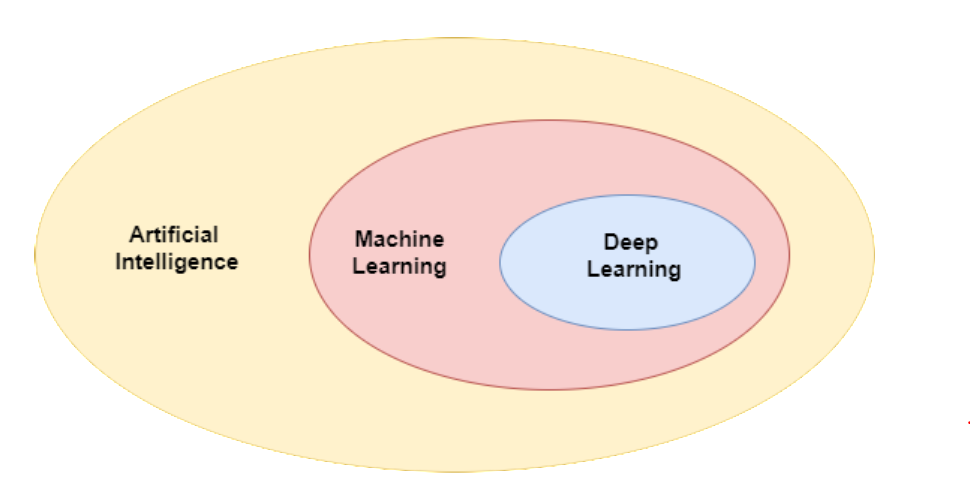
\includegraphics[scale=0.3]{./Figures/ai_ml_dl.png}
	\caption{Diagrama en bloques del sistema.}
	\label{fig:sys_blocks}
\end{figure}

explicar el funcionamiento...

\subsection{Placa de desarrollo ESP32-S3-DevKitC-1}
El componente central del sistema es la tarjeta de desarrollo ESP32-S3-DevKitC-1-N8R8 de la empresa Espressif. Tiene como componente central el modulo ESP32-S3-WROOM-1-N8R8 y varios otros componentes que simplifican el proceso de desarollo de aplicaiones para IoT. En la figura \ref{fig:devkit_comp} se observa una fotografia de la tarjeta con el detalle de sus componentes.

\begin{figure}[h]
	\centering
	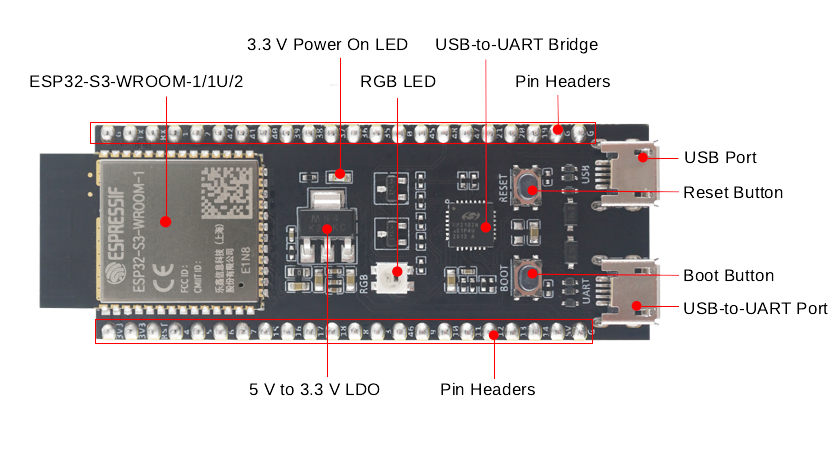
\includegraphics[scale=0.4]{./Figures/devkit_comp.png}
	\caption{Componentes del ESP32-S3-DevKitC-1.}
	\label{fig:devkit_comp}
\end{figure}

El modulo ç-WROOM-1-N8R8 es un potente modulo MCU (\textit{Microcontroller Unit}, Unidad de Microcontrolador) de doble nucleo que incorpora Wi-Fi y BLE (\textit{Bluetooth Low Energy}, Bluetooth de Baja Energia) y tiene un amplio conjunto de perifericos. Sus especificaciones tecnicas mas relevantes se detallan en la tabla \ref{tab:devkit_specs}.

\begin{table}[h]
	\centering
	\caption[ESP32-S3-DevKitC-1 especificaciones]{Tabla de especificaciones del ESP32-S3-DevKitC-1}
	\begin{tabular}{lc}    
		\toprule
		\textbf{Caracteristica} 	 & \textbf{Descripcion}  \\
		\midrule
		SoC embebido & ESP32-S3R8 \\
		Procesador & Xtensa LX7 doble nucleo de 32 bits \\
		Frecuencia & Hasta 240 MHz \\
		ROM & 384 KB \\
		SRAM & 512 KB \\
		Pines & 41 \\
		Flash & 8 MB \\
		PSRAM & 8 MB \\
		Tipo de antena & PCB \\
		Wi-Fi & 802.11 b/g/n hasta 150 Mbps \\
		Bluetooth & Bluetooth 5 y Bluetooth \textit{mesh} \\
		Perifericos & \begin{tabular}{@{}c@{}} GPIO, I2C, SPI, interfaz LCD, \\ interfaz de camara, UART, I2S, USB, PWM, ADC, \\ sensor tactil, sensor de temperatura, timer y \textit{watchdogs} \end{tabular} \\
	 	Rango de temeperatura &  –40 \textcelsius a 65 \textcelsius \\
		\bottomrule
		\hline
	\end{tabular}
	\label{tab:devkit_specs}
\end{table}

En el mercado existen muchos fabricantes que ofrecen tarjetas de desarrollo de caracteristicas tecnicas que podrian haber sido utilizadas para el desarrollo de este trabajo. Sin ir muy lejos, Espressif, fabricante de la ESP32-S3-DevKitC-1-N8R8, tiene toda una familia de modulos y tarjetas muy similares entre si. La eleccion de esta tarjeta en particular responde a los siguientes criterios:
\begin{itemize}
	\item Costo: Espressif ofrece en todos sus SoCs, modulos y tarjetas, un costo muy contenido por la gran cantidad de caracteristicas ofrecidas.
	\item Redes neuronales: la serie de SoCs ESP32-S3 ofrece soporte para instrucciones vectoriales, que acelera las tareas de computacion de redes neuronales. Esta fue la caracteristica mas importante al momento de la eleccion de esta tarjeta.
	\item Memoria: como el trabajo implicaba el uso de una camara y por tanto el manejo de \textit{buffers} de memoria de gran tamano para manipular las imagenes obtenidas, la cantidad de memoria externa que ofrecia esta tarjeta la hizo optima para la aplicacion. 
\end{itemize}

\subsection{Sensor de movimiento PIR}
Un sensor de movimiento PIR basa su funcionamiento al detectar diferencias en la energia IR (\textit{Infrared}, Infrarojo) en el campo de vision del sensor. Debido a que la senal de salida generada por el sensor es muy pequena, es necesario aplicar etapas de amplificacion y filtrado para elevar el nivel de tension de la senal de salida y al mismo tiempo filtrar el ruido que puede generar eventos falsos positivos. Esta salida analogica luego se debe convertir en una senal digital mediante la operacion de comparacion de ventanas y se puede utilizar, por ejemplo, como una interrupcion en un MCU. En la figura \ref{fig:move_blocks} se muestra el diagrama en bloques del sensor de movimiento PIR.

\begin{figure}[h]
	\centering
	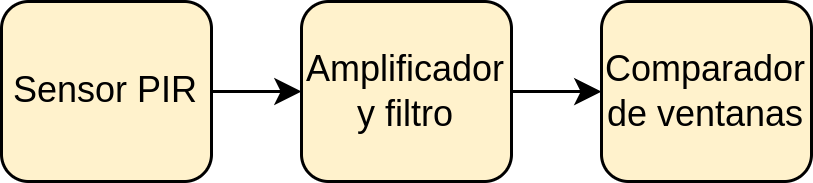
\includegraphics[scale=0.4]{./Figures/move_blocks.png}
	\caption{Diagrama en bloques del sensor de movimiento PIR.}
	\label{fig:move_blocks}
\end{figure}

\subsubsection{Sensor IRA-S230ST01}
El IRA-S230ST01 es un sensor PIR fabricado por la empresa Murata. Posee una alta sensibilidad y un rendimiento confiable gracias a la tecnologia ceramica y la tecnia de IC (\textit{Integrated Circuit}, Circuito Integrado) hibrida de Murata. Tiene ademas una sensibilidad mejorada a la interferencia de RF (\textit{Radio Frequency}, Radiofrecuencia). Sus aplicaciones mas comunes incluyen sistemas de seguridad, aparatos de iluminacion, electrodomesticos, entre otros. En la figura \ref{fig:pir_photo} se puede obsevar una fotografia del IRA-S230ST01.

\begin{figure}[h]
	\centering
	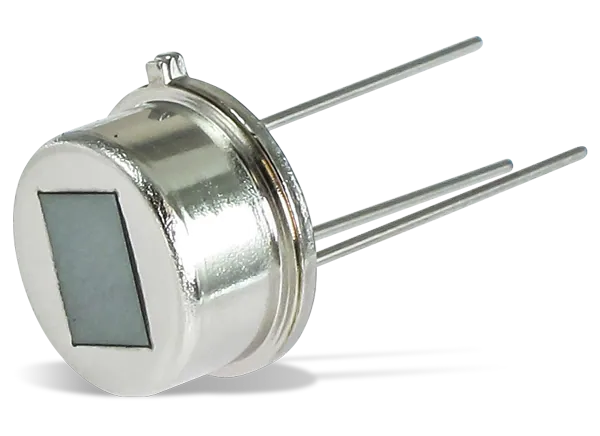
\includegraphics[scale=0.3]{./Figures/pir_photo.png}
	\caption{Fotografia del sensor IRA-S230ST01.}
	\label{fig:pir_photo}
\end{figure}

En la tabla \ref{tab:pir_specs} se detallan sus caracterisiticas tecnicas mas importantes.

 \begin{table}[h]
	\centering
	\caption[IRA-S230ST01 especificaciones]{Tabla de especificaciones del IRA-S230ST01}
	\begin{tabular}{lc}    
		\toprule
		\textbf{Caracteristica} 	 & \textbf{Descripcion}  \\
		\midrule
		Rango de temperatura & -40 \textcelsius a 70 \textcelsius\\
		SNR & 40 dB \\
		Campo de vision & theta1=theta2=45 grados \\
		Electrodo & (2.0x1.0mm)x2 \\
		Responsividad & 4.6 mV \\
		Filtro optico & 5 \textmu m paso alto \\
		Fuente de alimentacion & 2 V a 15 V \\
		\bottomrule
		\hline
	\end{tabular}
	\label{tab:pir_specs}
\end{table}

La eleccion del IRA-S230ST01 como sensor PIR responde a los siguientes criterios:
\begin{itemize}
	\item Marca: Murata es una marca muy reconocida en el mundo de los semiconductores y ofrece productos de muy alta calidad.
	\item Documentacion: el IRA-S230ST01 cuenta con docuemntacion muy clara sobre sus caracteristicas tecnicas.
\end{itemize}

\subsubsection{Amplificador operacional TVL8544}
El TLV8544 es un amplificador operacional cuadruple de ultra bajo consumo energetico de la empresa Texas Instruments, de costo optimizado para aplicaciones de sensado en equipos inalambricos y cableados de bajo consumo. El diseno del TLV8544 minimiza el consumo energetico en dispotiviso como sensores de movimiento para sistemas de seguridad, donde el tiempo de vida de la bateria que los alimenta es critico. Su uso mas comun es en configuraciones de amplificadores de transimpedancia con resitencias de \textit{feedback} en el orden de los Mega ohms. Adicionalmente, tiene proteccion contra EMI (\textit{Electromagnetic Interferencia}, Interferencia Electromagnetica) que reduce la sensibilidad a las senales de RF no deseadas de fuentes como telefonos moviles, Wi-Fi y transmisores de radio. En la figura \ref{fig:opamp_photo} se puede observar una fotografia del TLV8544 en un encapsulado TSSOP-14.

\begin{figure}[h]
	\centering
	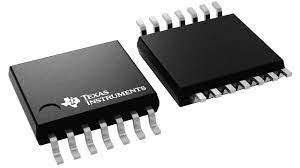
\includegraphics[scale=0.4]{./Figures/opamp_photo.jpeg}
	\caption{Fotografia del TLV8544 en un encapsulado TSSOP-14.}
	\label{fig:opamp_photo}
\end{figure}

Las caracterisiticas tecnicas mas importantes del TLV8455 se presentan en la tabla \ref{tab:opamp_specs}.

 \begin{table}[h]
	\centering
	\caption[TLV8544 especificaciones]{Tabla de especificaciones del TLV8544}
	\begin{tabular}{lc}    
		\toprule
		\textbf{Caracteristica} 	 & \textbf{Descripcion}  \\
		\midrule
		Numero de canales & 4 \\
		Fuente de alimentacion & 1.7 V a 3.6 V \\
		Corriente de salida por canal & 30 mA \\
		Corriente de operacion & 500 nA \\
		CMMR (\textit{Common Mode Rejection Ratio}, \\ Relacion de Rechazo del Modo Comun) & 90 dB \\
		Rango de temperatura & -40 \textcelsius  a 125 \textcelsius\\
		Corriente de polarizacion & 100 fA \\
		Ancho de banda de ganancia & 8 kHz \\
		\bottomrule
		\hline
	\end{tabular}
	\label{tab:opamp_specs}
\end{table}

Desde hace muchos anos los amplificadores operacionales son un dispositivos muy utilizada y en el mercado existen muchas empresas que los fabrican y muchos modelos existentes. Estos son los criterios de eleccion del TLV8544 para el presente trabajo:
\begin{itemize}
	\item Aplicacion: por sus caracterisiticas tecnicas, el TL8544 esta disenado para ser parte de las etaspas de amplificacion y filtrado en el diseno de un sensor de movimiento PIR.
	\item Documentacion: Texas Instruments, ademas del correspondiente \textit{datasheet} del TLV8544, ofrece varios docuemntos tecnicos con ejemplos de diseno para el TLV8544.
	\item Costo: es un dispositivo de precio muy razonable por todas las caracteristicas que ofrece.
	\item Cosumo energetico: con sus 500 nA de corriente de funcionamiento por canal, el TLV8544 es una opcion ideal para aplicaciones que requieran el uso de baterias.
\end{itemize}

\subsection{Cámara OV2640}
Otro de los componentes principales del sistema es la camara, que permite obtener imagenes en un formato digital que posteriormente deben ser procesadas por los algoritmos de DL. Para este trabajo se utilizo el modulo ESP-LyraP-CAM. Este modulo integra un CCM (\textit{Compact Camera Module}, Modulo de Camara Compacto) con un sensor OV2640 en conjunto con dos reguladores de tension para su correcto funcionamiento. En la figura \ref{fig:camera_blocks} se puede observar unas fotografias del modulo ESP-LyraP-CAM y sus componentes.

\begin{figure}[h]
	\centering
	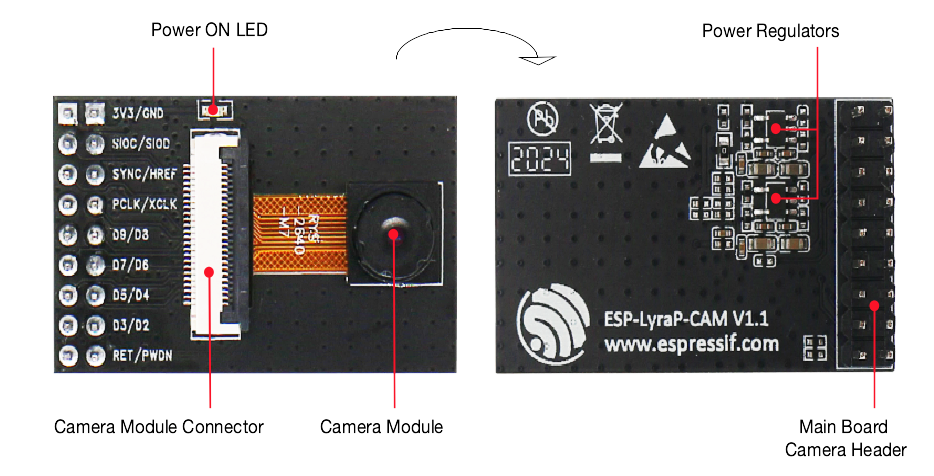
\includegraphics[scale=0.5]{./Figures/camera_blocks.png}
	\caption{Diagrama en bloques del del modulo ESP-LyraP-CAM.}
	\label{fig:camera_blocks}
\end{figure}

El OV2640 de la empresa OmniVision es un sensor CMOS (\textit{Complementary Metal-Oxide-Semiconductor}, Semiconductor de Oxido de Metal Complementario) de 2 MP, cuenta con una interfaz de comunicacion compatible con DVP  (\textit{Digital Video Port}, Puerto de Video Digital), soporta codificacion JPEG (\textit{Joint Photographic Experts Group}, Grupo Unido de Expertos en Fotografia) y es de bajo consumo energetico. En la tabla \ref{tab:ov2640_specs} se muestran las caracterisiticas tecnicas mas importantes del OV2640.

 \begin{table}[h]
	\centering
	\caption[OV2640 especificaciones]{Tabla de especificaciones del OV2640}
	\begin{tabular}{lc}    
		\toprule
		\textbf{Caracteristica} 	 & \textbf{Descripcion}  \\
		\midrule
		Tamano de matriz & 1600x1200 (UXGA) \\		
		Fuente de alimentacion & \begin{tabular}{@{}c@{}} \textit{Core}: 1.3 V ± 5\% \\ \textit{Analog} 2.5 ~ 3.0 V \\ I/O: 1.7 V - 3.3 V\end{tabular} \\
		Consumo energetico & \begin{tabular}{@{}c@{}} \textit{Free running}: 125 mW \\ \textit{Standby}: 600 \textmu A \end{tabular} \\
		Formato de imagen del sensor & 1/4'' \\
		Tasa de transferencia maxima & \begin{tabular}{@{}c@{}} 1600×1200 a 15 fps \\ SVGA a 30 fps \\ CIF a 60 fps \end{tabular} \\
		Sensibilidad & 0.6 / Lux-sec \\
		SNR & 40 dB \\
		Rango dinamico & 50 dB \\
		Tamano de pixel & x2.2x2.2 \textmu m \\
		Formato de salida & YUV/RGB/MJPEG \\
		\bottomrule
		\hline
	\end{tabular}
	\label{tab:ov2640_specs}
\end{table}

Los criterios para utilizar este modulo como camara del sistema son los siguientes:
\begin{itemize}
	\item Costo: los modulos con el sensor OV2640 tienen un costo muy reducido en comparacion con otros disponibles en el mercado.
	\item Bajo consumo energetico: como se mostro en la tabal \ref{tab:ov2640_specs} el consumo energetico del modulo en modo \textit{standby} es lo suficientemente bajo como para funcionar alimentado por baterias.
	\item Disponibilidad de codigo: al ser un modulo que ya lleva mucho tiempo en el mercado existen muchas bibliotecas de codigo para utilizarlo, lo que simplifica en gran medida el tiempo de desarrollo de \textit{firmware}.
\end{itemize}

%----------------------------------------------------------------------------------------
\section{MTCNN (\textit{Multi-Task Cascaded Convolutional Networks}, Redes Convolucionales en Cascada Multitarea)}
MTCNN es un \textit{framework} basado el el \textit{paper} Joint Face Detection and Alignment using Multi-task Cascaded Convolutional Networks” by Zhang, Zhang and Zhifeng, esta desarrollado para integrar las tareas de deteccion facial y alineamiento facial con ayuda de CNNS en cascada mediante aprendizaje multitarea. El proceso consta de tres etapas de CNNs que puede detectar rostros humanos, sus posiciones y las posiciiones de sus rasgos faciales (nariz, ojos y boca). En la figura \ref{fig:mtcnn_pipe} se muestra el \textit{pipeline} utilizado en MTCNN.

\begin{figure}[h]
	\centering
	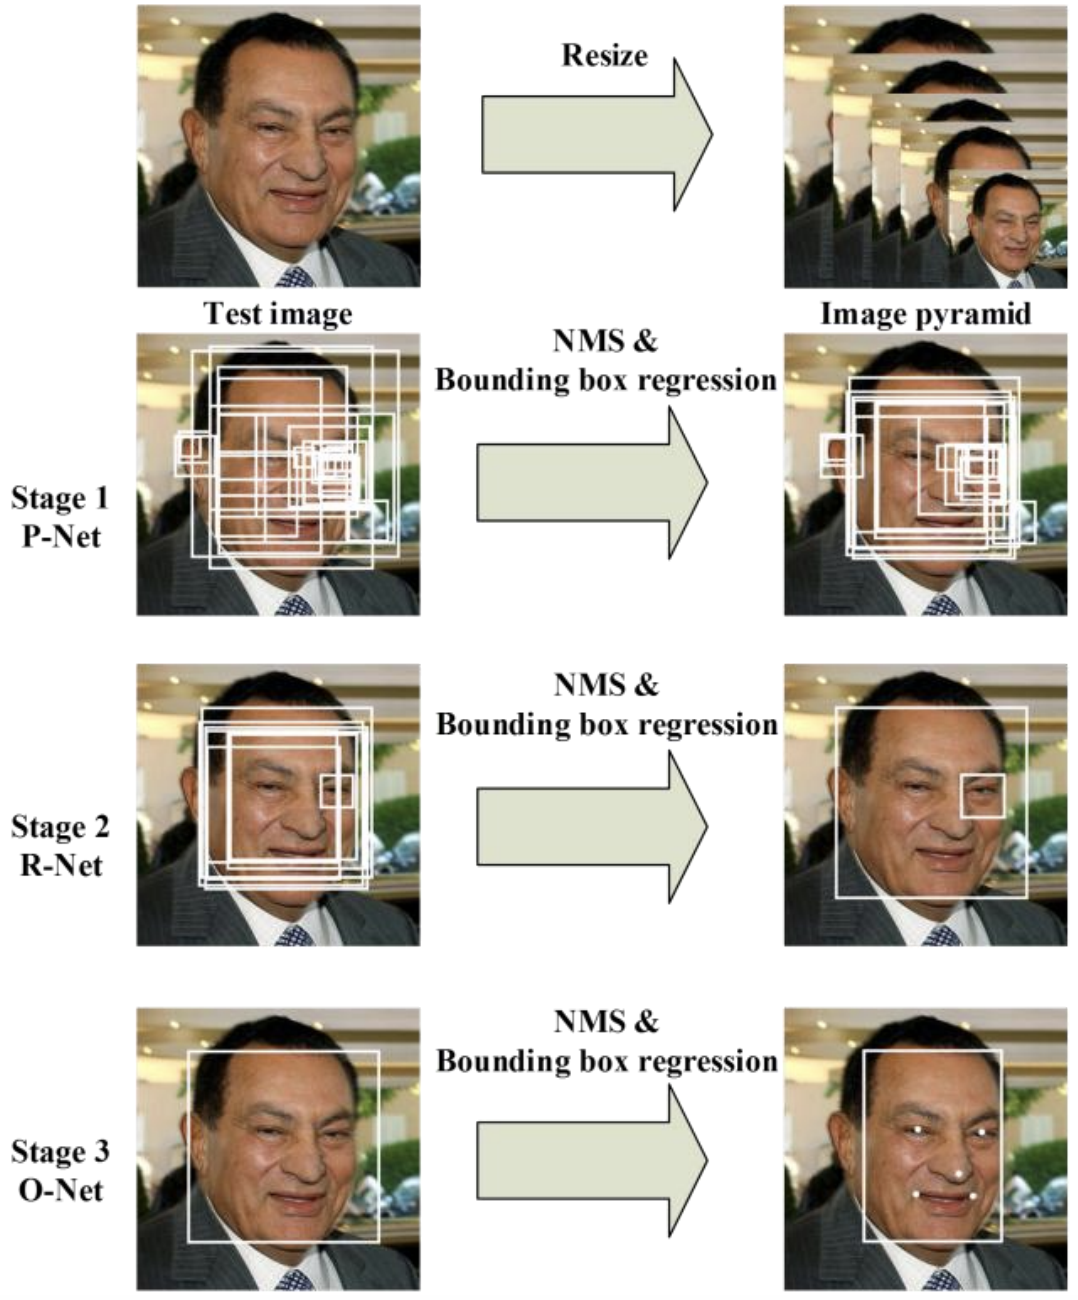
\includegraphics[scale=0.5]{./Figures/mtcnn_pipe.png}
	\caption{\textit{Pipeline de MTCNN}.}
	\label{fig:mtcnn_pipe}
\end{figure}

El \textit{pipeline} de la figura \ref{fig:mtcnn_pipe} indica que las imagenes de entrada deben ser reducidas de tamano en varias escalas para formar un piramide de imagenes, que serviran para alimentar las siguientes tres etapas de MTCNN

\subsection{P-Net}
Tambien conocida como \textit{Proposal Network} o red de propuestas, esta etapa esta compuesta de una FCN (\textit{Fully Convolutional Network}, Red Totalmente Convolucional). La diferencia entre una FCN y una CNN es que la FCN no utiliza una capa FC como parte de su arquitectura. Tiene la funcion de obtener ventanas candidatas y sus vectores de regresion de \textit{bounding box}. La regresion de \textit{bounding box} es una tecnica para predecir la localizacion de un cuadro delimitador en el que se encuentra el objeto que quiere ser detectado, en este caso rostros humanos. Una vez que se obtienen estos vectores, se realizan una operacion conocida como NMS (\textit{Non Max Supression}, Supresion no Maxima) para combinar las regiones sobrepuestas entre si. Finalmente las ventanas candidatas resultantes pasan a la siguiente etapa. En la figura \ref{fig:mtcnn_pnet} se muestra la arquitectura de P-Net.

\begin{figure}[h]
	\centering
	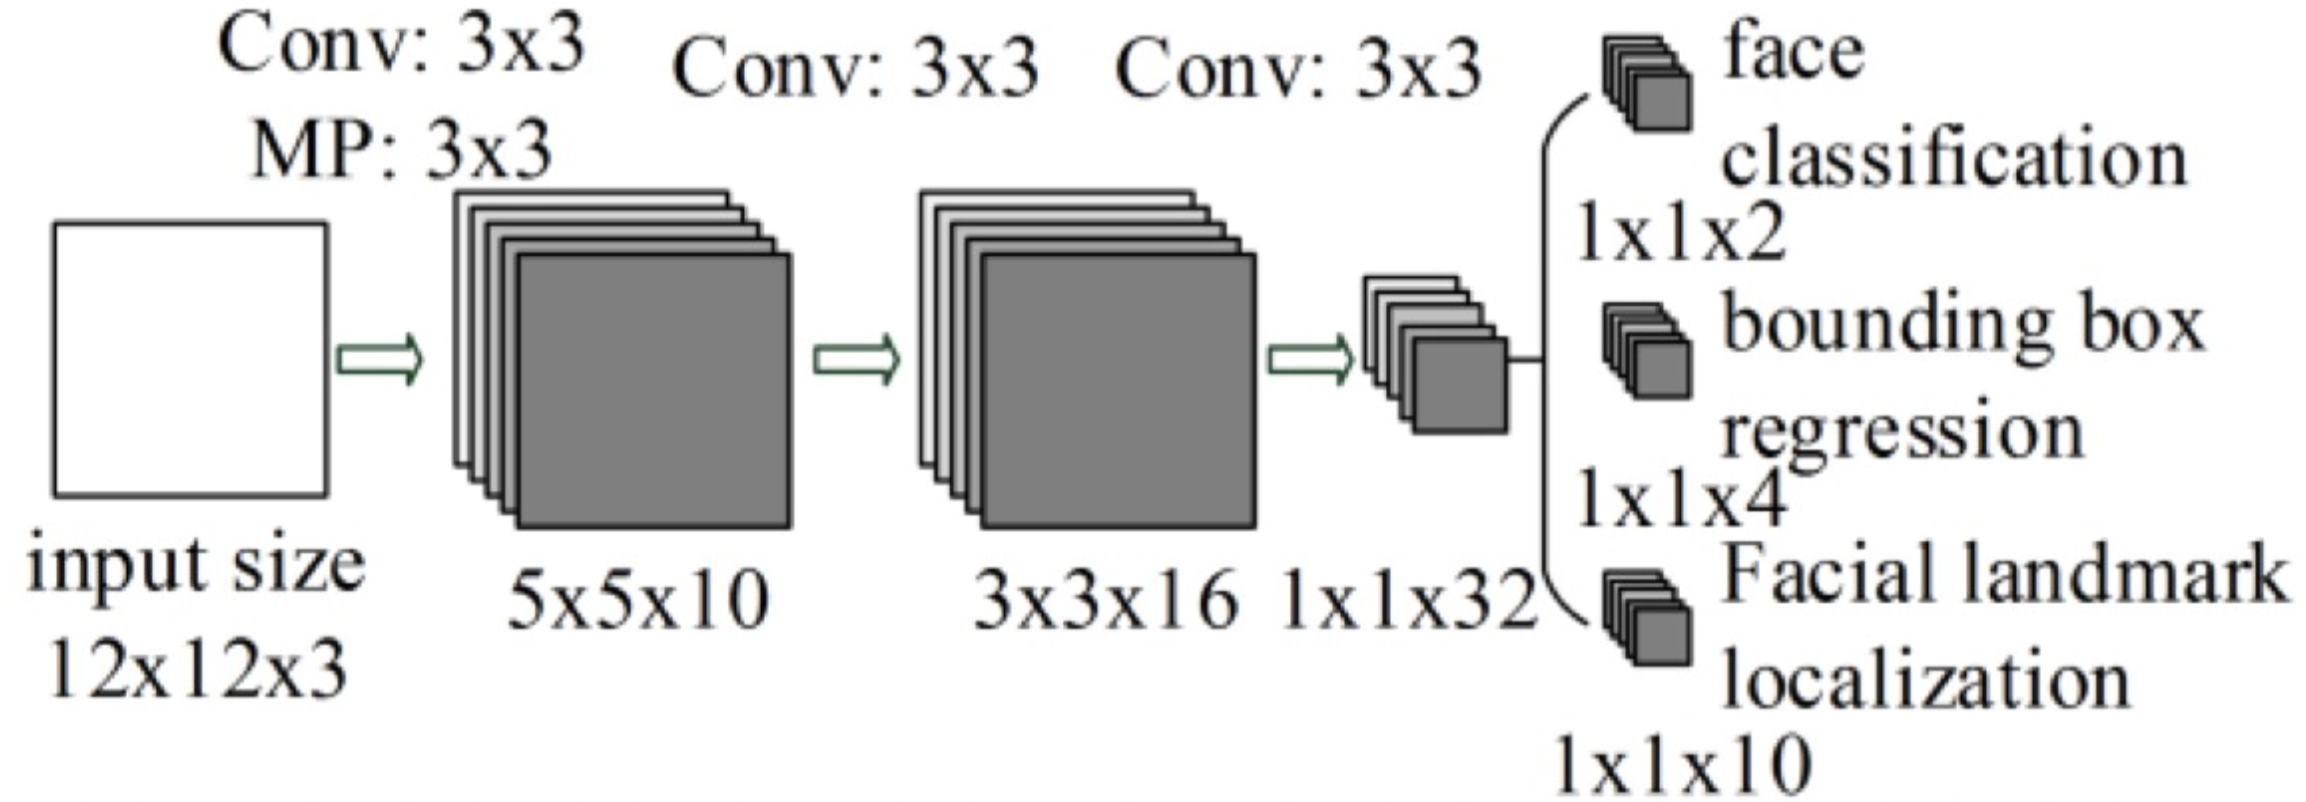
\includegraphics[scale=0.25]{./Figures/mtcnn_pnet.png}
	\caption{\textit{Arquitectura de P-Net}.}
	\label{fig:mtcnn_pnet}
\end{figure}
	
\subsection{R-Net}
Esta es una CNN denominada \textit{Refine Network} o red de refinamiento. Los candidatos provenientes de P-Net son la entrada de esta red. La arquitectura de R-Net reduce aun mas el numero de candidatos, realiza la calibracion con regresion de \textit{bounding box} y emplea NMS para fusionar candidatos superpuestos. Para cada candidato de entrada, R-Net obtiene la probabilida de si es un rostro o no, un vector de 4 elementos que es el \textit{bounding box} y un vector de 10 elementos que represetan la locacliacion de rasgos faciales. En la figura \ref{fig:mtcnn_rnet} se muestra la arquitectura de R-Net.

\begin{figure}[h]
	\centering
	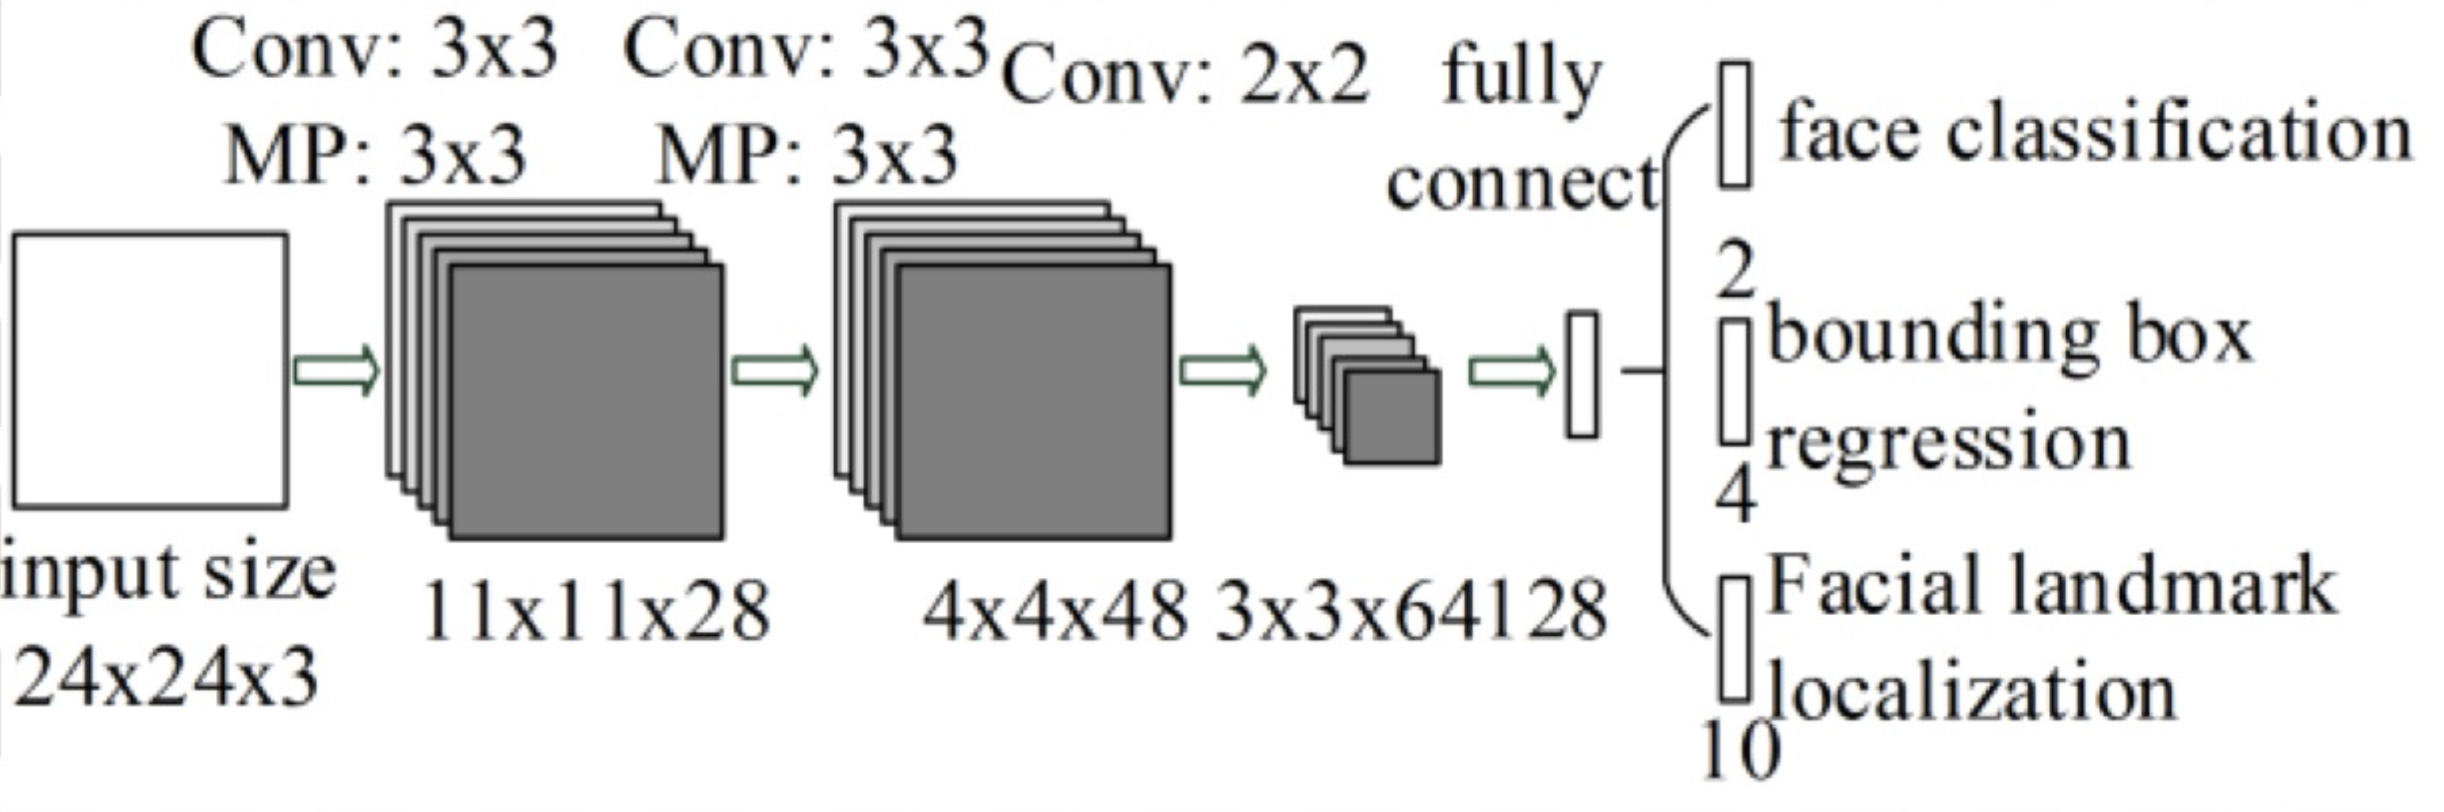
\includegraphics[scale=0.25]{./Figures/mtcnn_rnet.png}
	\caption{\textit{Arquitectura de R-Net}.}
	\label{fig:mtcnn_rnet}
\end{figure}

\subsection{O-Net}
Conocida como \textit{Output Network} o red de salida, es muy similar a R-Net, pero esta enfocada a describir el rostro con mas detalle y generar las cinco localizaciones para ojos, boca y nariz. Su arquitectura se muestra en la figura \ref{fig:mtcnn_onet}.

\begin{figure}[h]
	\centering
	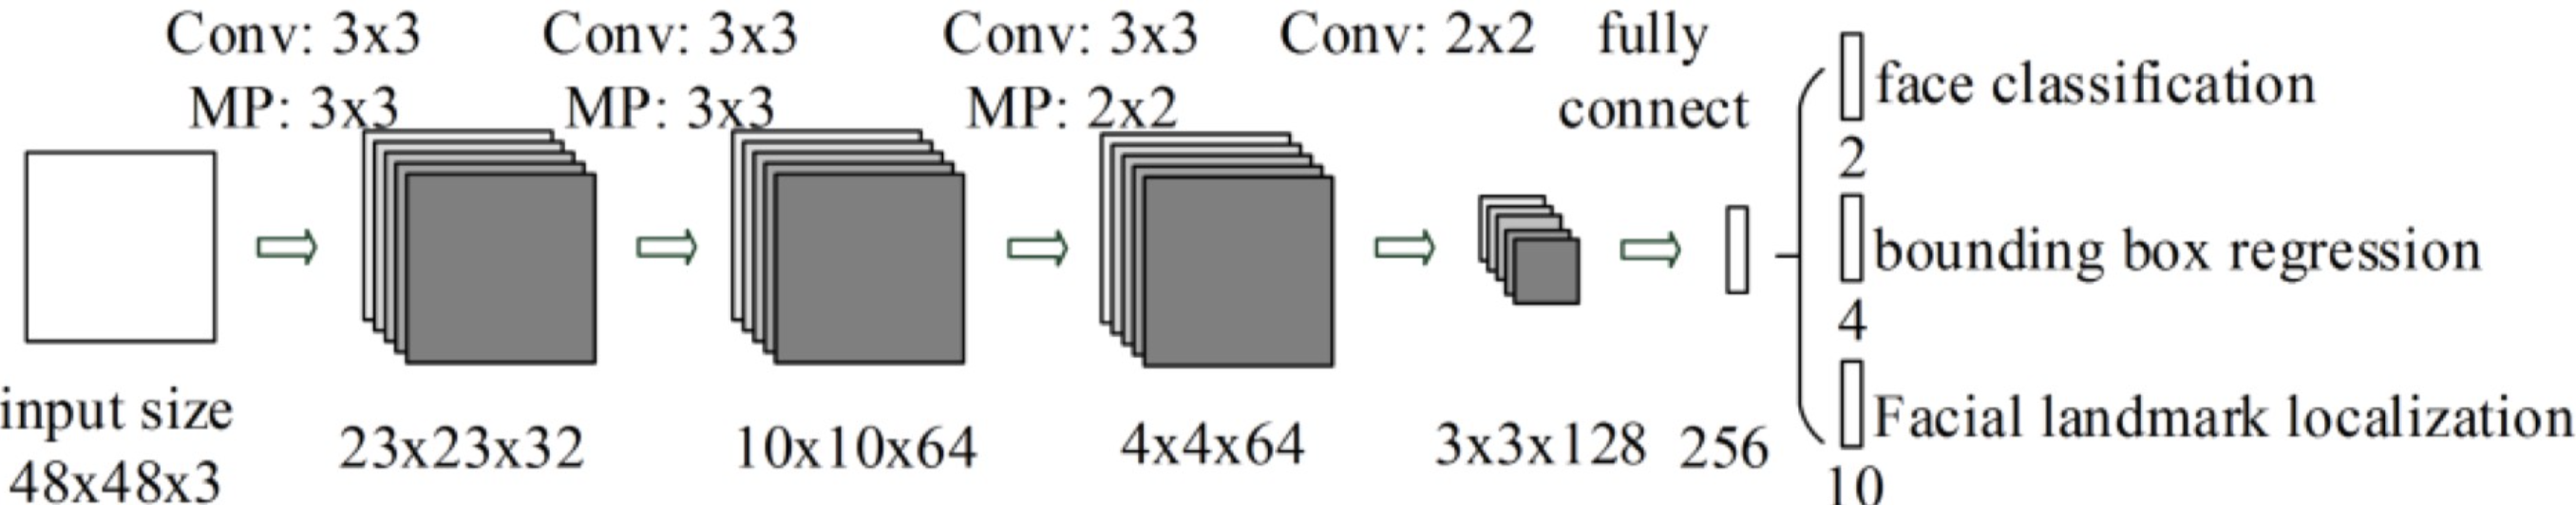
\includegraphics[scale=0.3]{./Figures/mtcnn_onet.png}
	\caption{\textit{Arquitectura de O-Net}.}
	\label{fig:mtcnn_onet}
\end{figure}

\subsection{Tareas de MTCNN}
Como se explico en los puntos anteriores, MTCNN se compone de tres etapas que filtran ventanas candidatas y con la ayuda de NMS y calibracion con los vectores de regresion de \textit{bounding box}, se detectan rostros y sus rasgos. Entonces, el proposito de MTCNN es cumplir con las siguientes tareas:
\begin{itemize}
	\item Clasificacion rostro/no rostro: este es un problema de clasificacion binaria que utiliza una funcion de perdida de entropia cruzada. 
	\item Regresion de \textit{bounding box}: el objetivo de aprendizaje es un problema de regresion. Para cada candidato, se calcula el \textit{offset} entre el candidato y el \textit{ground thrut} [ref] mas cercano. La funcion de perdida Euclidiana es uitilizada para esta tarea.
	\item Localizacion de rasgos faciales:es formulada como un problema de regresion en el que la funcion de perdida es la distancia Euclidiana.
\end{itemize}

%----------------------------------------------------------------------------------------
\section{TensorFlow}
TensorFlow es una plataforma de codigo abierto para ML. Tiene un ecosistema completo y flexible de herramientas, bibliotecas y recursos comunitarios que permite a los desarrolladores crear e implementar fácilmente aplicaciones basadas en ML.

Fue originalmente desarrollador por investigadores e ingenieros que trabajaban en el equipo Google Brain dentro de la organizacion de investigacion de inteligencia artificial de Google y la version inicial fue lanzaeda en 2015 bajo la licencia Apacha License 2.0 [https://github.com/tensorflow/tensorflow].

TensorFlow proporciona APIs estables y oficiales para Python y C++, aunque tambien existen APIs para otros lenguajes de programacion que no estan garantizadas de manera oficial.

Sus caracterisiticas principales son:
\begin{itemize}
	\item Autodiferenciacion: es el proceso de calculo automatico del vector gradiente de un modelo respecto a cada uno de sus parametros.
	\item Ejecucion ansiosa: significa que las operaciones se evaluan de manera inmediata en lugar de agregarse a un grafico computacional que se ejecuta mas tarde.
	\item Distribuido: TensrFlow proporciona una API para distribuir el computo en multiples dispositivos tanto para ejecucion ansiosa como para graficos computacionales.
	\item Perdidas: TensorFlow proporciona un conjunto de funciones de perdida, tambien conocidas como funciones de costo.
	\item Metricas: TensorFlow brinda acceso a un API de metricas de uso comun que se utilizan para evaluar el rendimiento de los modelos de ML.
	\item Optimizadores: TensorFlow ofrece un conjunto de optimizadores para entrenar redes nuronales, algunos son ADAM, ADAGRAD y SGD (\textit{Stochastic Gradient Descent}, Descenso de Gradiente Estocastico).
\end{itemize} 

Para el desarrollo de aplicaciones de ML existen varias otras bibliotecas, algunas de las mas populares son: PyTorch, Caffe Computer Vision Library, Deeplearning, Neuroph, OpenNN, Theano, Torch y MXNet. Los criterios de eleccion de TensorFlow en este trabajo sobre las anteriores bibliotecas citadas fueron:
\begin{itemize}
	\item Experiencia: este fue el criterio mas fuerte en eleccion de TensorFLow como \textit{framework} para el desarrollo de modelos de ML. El autor de este trabajo ya poseia experiencia trabajando con TensorFlow.
	\item Documentacion: TensorFlow tiene mucha documentacion oficial sobre su API y una gran varieda de tutoriales de uso.
	\item Herramientas para cuantizacion: TensorFlow cuenta con herramientas de cuantizacion de datos para optimizar el tamano y tiempos de ejecucion de modelos de ML.
\end{itemize}

%----------------------------------------------------------------------------------------
\section{AWS (\textit{Amazon Web Services}, Servicios Web de Amazon)}
AWS es una plataforma de \textit{cloud computing} provista por Amazon que incluye una combinacion de IaaS, PaaS y SaaS. Los servicios de AWS pueden ofrecer herramientas de poder computo, almacenamiento de datos y servicios de entrega de contenido.

AWS esta dividido en distintos tipos de servicios que pueden ser configurados segun las necesidades de cada usuario. Estos servicios puede dividirse en las siguientes categorias: computacion, almacenamiento, bases de datos, administracion de datos, migracion, redes, herramientas de desarrollo, monitoreo, administracion de \textit{big data}, analiticas, AI, desarrollo movil, mensajeria y notificaciones.

De todos la extensa cantidad de servicios que ofrece AWS, para este trabajo se necesitaron solo los siguientes: IoT Core y Amazon Timestream.

\subsection{IoT Core}
Proporciona los servicios en la nube necesarios para conectar dispositivos IoT entre si y a los servicios a otros servicios de AWS. En la figura \ref{fig:aws_iot} se puede observar un diagrama de interconexion de dispositivos IoT y los servicios de AWS mediante IoT Core. 

\begin{figure}[h]
	\centering
	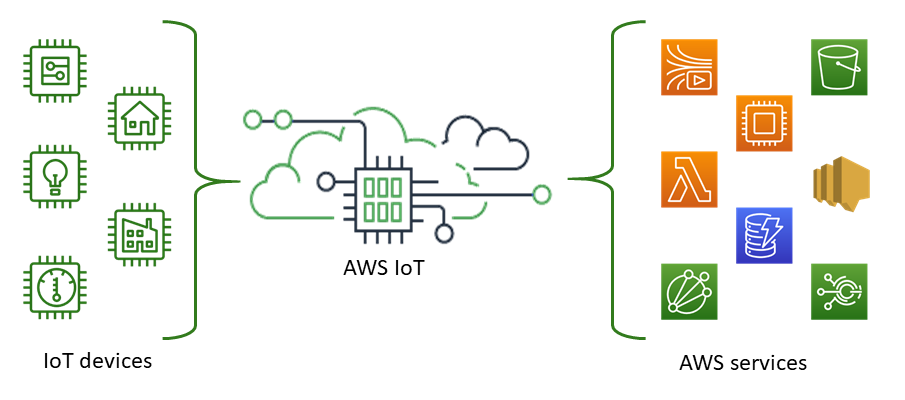
\includegraphics[scale=0.5]{./Figures/aws_iot.png}
	\caption{Diagrama de conexion entre dispositivos IoT y AWS.}
	\label{fig:aws_iot}
\end{figure}

IoT Core permite seleccionar las tecnologias mas acdecuadas y actualizadas para interconectar dispositivos IoT. Los protocolos de comunicacion soportados son: MQTT (\textit{Message Queuing and Telemetry Transport}, Cola de Mensajes y Transporte de Telemetria), MQTT sobre WSS (\textit{Websocket Secure}, Webscoket Seguro), HTTPS (\textit{Hypertext Transfer Protocol Secure}, Protocolo de Transferencia de Hipertexto Seguro) y LoRaWAN.

El \textit{broker} de IoT Core admite dispositivos y clientes que ulitizan MQTT y MQTT sobre WSS para publicar y suscribirse a algun topico. Tambien es compatible con dispositivos y clientes que utilizan HTTPS para publicar mensajes.

\subsection{Amazon Timestream}
Amazon Timestream es una base de datos de series temporales rapida, escalable y totalmente administrada, que facilita el almacenamiento y el analisis de billones de datos de series temporales al dia. Timestream ahorra tiempos y costos con su capacidad de administrar los ciclos de vida de los datos de series temporales, donde mantiene los datos recientes en la memoria y mueve los datos historicos a un nivel de almacenamiento optmizado segun las politicas definidas previamente por el usuario. El motor de consultas de Timestream permite acceder y analizar datos reciente e historicos al mismo tiempo. No necesita servidor y su tamano se acomoda automaticamente para ajustar la capacidad y el rendimiento requeridos. 

Los beneficios mas notables que ofrece Amazon Timestream son:
\begin{itemize}
	\item Sin servidor con escalado automatico: a medida que cambian las necesidades de la palicacion, Timestram escala automaticamente para ajustar la capacidad.
	\item Administracion de los ciclos de vida de los datos: ofrece ofrece niveles de almacenamiento, con un almacenamiento de memoria para datos recientes y un almacenamiento magnetico para datos historicos. Timestream automatiza el proceso de transferencia entre ambos almacenamientos.
	\item Acceso simplificado a los datos: el motor de consultas de Timestream permite acceder a los datos de forma transparente, sin la necesidad de especificar el nivel de almacenamiento.
	\item Disenado para series temporales: puede analizar datos de series de tiempo con SQL, con funciones integradas de series de de tiempo para suavizar, aproximar e interpolar.
	\item Siempre cifrado: garantiza que los dato de series de tiempo siempre esten cifrados. Timestream permite especificar una clave administrada para encriptar datos en el almacenamiento magnetico.
	
\end{itemize}

%----------------------------------------------------------------------------------------
\section{Grafana}
Es una aplicacion web multi plataforma de analisis y visualizacion interactiva. Proporciona tablas, graficos y alertas a traves de la web cuando se conecta a alguna fuente de datos compatible. Los usuarios pueden crear \textit{dashboards} de monitoreo de datos complejos con ayuda de generadores de consultas interactivos.

Como herramienta de visualizacion, Grafana es muy popular gracias a las siguientes caracteristicas:
\begin{itemize}
	\item Se conecta a muchas fuentes de datos populares como Graphite, Prometheus, Influx DB, ElasticSearch, MySQL, PostfreSQL, entre otros.
	\item Es de codigo abierto y distribuida bajo la licencia  AGPL-3.0, que permite desarrollar complementos desde cero para integrarla con otras fuentes de datos.
	\item Ayuda a estudiar, analizar y monitorear datos durante un periodo de tiempo condifurable por el usuario.
	\item Puede ser implementado localmente por organizaciones que quieran mantener sus datos confidenciales sin acceso a internet.
	\item Se pueden configurar alertas que se envian por otros medios de comunicacion bajo ciertas condiciones pre establecidas.
\end{itemize}

